%%%%%%%%%%%%%%%%%%%%%%%%%%%%%%%%%%%%%%%%%%%%%%%%%%%%%%%%%%%%%%%%%%%%%%%%
\chapter{Introduction}
%%%%%%%%%%%%%%%%%%%%%%%%%%%%%%%%%%%%%%%%%%%%%%%%%%%%%%%%%%%%%%%%%%%%%%%%

\begin{center}
  \begin{minipage}{0.5\textwidth}
    \begin{small}
      In which the reasons for doing this Ph.D. are laid bare for the whole world to see and we encounter some answers to questions in which, frankly, only an extremely small number of people were interested in the first place.
    \end{small}
  \end{minipage}
  \vspace{0.5cm}
\end{center}

\noindent This package contains a minimal, modern template for writing your
thesis. While originally meant to be used for a Ph.\,D.\ thesis, you can
equally well use it for your honour thesis, bachelor thesis, and so
on---some adjustments may be necessary, though.

\section{The BASNUM Project}

Cette thèse s'inscrit dans le cadre du projet ANR BASNUM (ANR-18-CE38-0003), qui avait comme objectif principal de numériser le Dictionnaire Universel (DU) d'Antoine Furetière, dans sa version de 1701 revue et corrigée par Basnage de Beauval \citep{furetiere-1701-dictionnaire}, et de l'analyser avec des outils numériques, afin de faire apparaître l'importance de cet ouvrage pour l'évolution des sciences et des mentalités au XVIIIe siècle. Le projet visait également à contribuer au mouvement actuel de conception de méthodes innovantes de numérisation, encodage et analyse des textes.

D'un point vue purement informatique le projet BASNUM comptait réaliser deux types de tâches :
\begin{enumerate}
  \item une première tâche de structuration où la macrostructure du dictionnaire serait annoté;
  \item une deuxième tâche d'enrichissement qui consistait à réaliser un large éventail de tâches d'extraction d'informations, d'annotation de la microstructure du dictionnaire et même de normalisation et modernisation du texte.
\end{enumerate}

La première tâche de structuration automatique des dictionnaires était déjà partiellement couverte par les travaux de \citet{khemakhem-etal-2017-automatic,khemakhem-etal-2018-enhancing} qui développent \emph{GROBID-dictionaries}, un sous-module de \emph{GROBID}\footnote{Bibliothèque d'apprentissage automatique pour extraire, analyser et restructurer des documents bruts tels que PDF, en documents structurés et encodés en TEI.} \citep{lopez-etal-2018-grobid} implémentant une bibliothèque d'apprentissage automatique Java pour la structuration de ressources lexicales numérisées au format \emph{TEI} \citep{tei-2018-guidelines}, afin de permettre l'analyse, l'extraction et la structuration d'informations textuelles dans de telles ressources. \emph{GROBID-dictionaries} avait déjà obtenu des résultats et des performances prometteurs \citep{khemakhem-2020-standard}, à tel point qu'il a été utilisé pour faire une première annotation de la macrostructure du Dictionnaire Universel.

Étant donnés les travaux réalisés par \citet{khemakhem-2020-standard}, nous avons décidé de nous concentrer sur la deuxième tâche d'enrichissement des dictionnaires, qui à l'époque restait assez générale et abstraite, notamment par contraste avec la première tâche de structuration. Pour aborder cette tâche, nous avions deux options: soit nous développions de multiples modèles et systèmes d'annotation dédiés à chacune des sous-tâches impliquées dans cet \emph{enrichissement} et ciblant très spécifiquement le Dictionnaire Universel, soit nous développions un seul modèle d'annotation générique capable d'aborder toutes les sous-tâches d'enrichissement et capable de traiter non seulement le Dictionnaire Universel, mais aussi d'autres textes et ressources de l'époque moderne\footnote{Entre le 16e et le 18e siècle.}.

Étant donnée la nature de la tâche d'enrichissement et le fait que de nouveaux modèles de langue neuronaux capables transférer des connaissances entre différentes tâches en traitement automatique du langage naturel (TALN) venaient d'être publiés au début de cette thèse \cite{peters-etal-2018-deep,devlin-etal-2019-bert}, nous avons décidé de nous concentrer sur la deuxième option et, en conséquence, de développer un seul modèle général que nous espérions capable d'être utilisé pour toutes ces tâches d'enrichissement et pour n'importe quel type de document en français moderne ou contemporain.

En choisissant cette approche, nous voulions aussi aborder d'une façon indirecte la première tâche de structuration automatique, parce que nous croyons qu'il était possible d'améliorer les premiers résultats de GROBID-dictionaries en utilisant des nouveaux modèles neuronaux. En effet GROBID-dictionaries reposait sur des modèles CRF (Champ aléatoire conditionnel) \cite{lafferty-etal-2001-conditional} qui étaient largement utilisés pour l'étiquetage et la classification des tokens, mais qui ont été remplacés par ces modèles neuronaux au cours des dernières années \citep{lample-etal-2016-neural,devlin-etal-2019-bert}. En outre, nous savions que les développeurs de GROBID avaient commencé à travailler avec certains de ces modèles neuronaux en écrivant \emph{DeLFT}, une bibliothèque pour le traitement de texte, couvrant l'étiquetage et la classification de tokens. Cette bibliothèque réimplémente les derniers modèles d'apprentissage automatique en TALN \citep{lopez-etal-2018-delft} et vise à améliorer les pipelines de \emph{GROBID}. Ce sont des outils et des idées comme ceux contenus dans \emph{DeLFT} qui pouvaient être appliqués à \emph{GROBID}-Dictionaries pour améliorer et étendre considérablement ses capacités au profit du projet \emph{BASNUM}, surtout en plus des ressources que nous avions décidé de développer.

Ayant choisi de développer ces nouveaux modèles pour le français, tels que \emph{ELMo} \citep{peters-etal-2018-deep} ou \emph{BERT} \cite{devlin-etal-2019-bert}, nous devions commencer par construire et rassembler notre propre corpus pour le pre-entraînement de ces architectures, puisque les corpus en français contemporain librement disponibles à l'époque, tels que Wikipedia ou frWAC \citep{baroni-etal-2009-the}, n'étaient pas considérés comme étant suffisamment grands pour cela \citep{liu-etal-2019-roberta}.

Notre plan était alors de développer un corpus de pre-entraînement en français contemporain, puis de pre-entraîner un modèle de langue pour le français contemporain et enfin d'utiliser les capacités de transfert de connaissances de ces architectures pour l'adapter au français moderne, au cas où nous ne serions pas en mesure de trouver assez de ressources textuelles pour pre-entrainer directement un tel modèle de langue pour le français moderne. Au cours de cette thèse, nous voulions également étudier la question de la quantité minimale de ressources requise pour pre-entraîner avec succès de telles modèles, quantité qui, à l'époque, était considérée comme plus élevée que ce qui est disponible pour les langues historiques \citep{peters-etal-2018-deep,liu-etal-2019-roberta}.

%%%%%%%%%%%%%%%%%%%%%%%%%%%%%%%%%%%%%%%%%%%%%%%%%%%%%%%%%%%%%%%%%%%%%%%%
\section{Language Modeling}
%%%%%%%%%%%%%%%%%%%%%%%%%%%%%%%%%%%%%%%%%%%%%%%%%%%%%%%%%%%%%%%%%%%%%%%%

In recent years neural methods for Natural Language Processing (NLP) have consistently and repeatedly improved the state-of-the-art in a wide variety of NLP tasks such as parsing, PoS-tagging, named entity recognition, machine translation, text classification and reading comprehension among others. Probably the main contributing factor in this steady improvement for NLP models is the raise in usage of \emph{transfer learning} techniques in the field. These methods normally consist of taking a pre-trained model and reusing it, with little to no retraining, to solve a different task from the original one it was intended to solve; in other words, one \emph{transfers} the \emph{knowledge} from one task to another.

Most of the transfer learning done in NLP nowadays is done in an unsupervised manner, that is, it normally consists of a  \emph{language model} that is fed unannotated plain text in a particular language; so that it \emph{extracts} or \emph{learns} the basic \emph{features} and patterns of the given language, the model is subsequently used on top of an specialised architecture designed to tackle a particular NLP task. Probably the best known example of this type of model are \emph{word embeddings} which consist of real-valued vector representations that are trained for each word on a given corpus. Some notorious examples of word embeddings are word2vec \citep{mikolov-etal-2013-distributed}, GloVe \citep{pennington-etal-2014-glove} and \mbox{fastText} \citep{mikolov-etal-2018-advances}. All these models are \emph{context-free}, meaning that a given word has one single vector representation that is independent of context, thus for a polysemous word like Washington, one would have one single representation that is reused for the city, the state and the US president.

In order to overcome the problem of polysemy, \emph{contextual} models have recently appeared. Most notably ELMo \citep{peters-etal-2018-deep} which produces deep contextualised word representations out of the internal states of a deep bidirectional language model in order to model word use and how the usage varies across linguistic contexts. ELMo still needs to be used alongside a specialised architecture for each given downstream task, but newer architectures that can be fine-tuned have also appear. For these, the model is first fed unannotated data, and is then fine-tuned with annotated data to a particular downstream task without relying on any other architecture. The most remarkable examples of this type of model are GPT-1, GPT-2 \citep{radford-etal-2018-improving,radford-etal-2019-language}, BERT \citep{devlin-etal-2019-bert} and XLNet \citep{yang-etal-2019-xlnet}; the latter being the current state-of-the-art for multiple downstream tasks. All of these models are different arrangements of the Transformer architecture \citep{vaswani-etal-2017-attention} trained with different datasets, except for XLNet which is an instance of the Transformer-XL \citep{dai-etal-2019-transformer}.

Even though these models have clear advantages, their main drawback is the amount of data that is needed to train them in order to obtain a functional and efficient model. For the first English version of word2vec, \citet{mikolov-etal-2013-distributed} used a one billion word dataset consisting of various news articles. Later \citet{al-rfou-etal-2013-polyglot} and then \citet{bojanowski-etal-2017-enriching} used the plain text from Wikipedia to train distributions of word2vec and fastText respectively, for languages other than English. Now, the problem of obtaining large quantities of data aggravates even more for contextual models, as they normally need multiple instances of a given word in order to capture all its different uses and in order to avoid overfitting due to the large quantity of hyperparameters that these models have. \citet{peters-etal-2018-deep} for example use a 5.5 billion token\footnote{Punctuation marks are counted as tokens.} dataset comprised of crawled news articles plus the English Wikipedia in order to train ELMo, \citet{devlin-etal-2019-bert} use a 3.3 billion word\footnote{Space sparated tokens.} corpus made by merging the English Wikipedia with the BooksCorpus \citep{zhu-etal-2015-aligning}, and \citet{radford-etal-2019-language} use a 40GB English corpus created by scraping outbound links from Reddit.\footnote{\url{https://www.reddit.com/}}

While Wikipedia is freely available, and multiple pipelines exist\footnote{\url{https://github.com/attardi/wikiextractor}}\textsuperscript{,}\footnote{\url{https://github.com/hghodrati/wikifil}} to extract plain text from it, some of the bigger corpora mentioned above are not made available by the authors either due to copyright issues or probably because of the infrastructure needed to serve and distribute such big corpora. Moreover the vast majority of both these models and the corpora they are trained with are in English, meaning that the availability of high quality NLP for other languages, specially for low-resource languages, is rather limited.

Pretrained word representations have a long history in Natural Language Processing (NLP), from non-contextual \citep{brown-etal-1992-class,ando-zhang-2005-framework,mikolov-etal-2013-distributed,pennington-etal-2014-glove} to contextual word embeddings \citep{peters-etal-2018-deep,akbik-etal-2018-contextual}. Word representations are usually obtained by training language model architectures on large amounts of textual data and then fed as an input to more complex task-specific architectures. More recently, these specialized architectures have been replaced altogether by large-scale pretrained language models which are \emph{fine-tuned} for each application considered. This shift has resulted in large improvements in performance over a wide range of tasks \cite{devlin-etal-2019-bert,radford-etal-2019-language,liu-etal-2019-roberta,raffel-etal-2020-exploring}.

These transfer learning methods exhibit clear advantages over more traditional task-specific approaches. In particular, they can be trained in an \emph{unsupervized} manner, thereby taking advantage of the information contained in large amounts of raw text.
Yet they come with implementation challenges, namely the amount of data and computational resources needed for pre-training, which can reach hundreds of gigabytes of text and require hundreds of GPUs \citep{yang-etal-2019-xlnet,liu-etal-2019-roberta}. This has limited the availability of these state-of-the-art models to the English language, at least in the monolingual setting. This is particularly inconvenient as it hinders their practical use in NLP systems. It also prevents us from investigating their language modelling capacity, for instance in the case of morphologically rich languages.


%%%%%%%%%%%%%%%%%%%%%%%%%%%%%%%%%%%%%%%%%%%%%%%%%%%%%%%%%%%%%%%%%%%%%%%%
\section{Digital Humanities and NLP for Historical Languages}
%%%%%%%%%%%%%%%%%%%%%%%%%%%%%%%%%%%%%%%%%%%%%%%%%%%%%%%%%%%%%%%%%%%%%%%%

% Context
There is a growing interest in digital humanities for automatic processing and annotation of historical texts. In this work, we study how to take advantage of current NLP models of the BERT family to advance the state of the art in processing historical languages, taking Old French (9th-13th century French) as a use case.

Old French is one of the historical languages for which we have the largest amount of syntactically annotated data, and we expect that our results on these language states may be generalised and used as a source of inspiration for researchers currently developing annotated resources for other historical languages.

Using contextual word embeddings as input representations has brought clear gains in performances for most of the NLP tasks for which they have been used.
However, this has mostly been attested in languages where sufficient (raw) linguistic data is available.
For less-resourced languages, the most common approach has been to leverage multilingual models such as mBERT \citep{devlin-etal-2019-bert}

Historical languages are typical cases where available linguistic data is limited, with no chance of acquiring new texts. They are also not normalized by spelling and institutional conventions and tend to be more heterogeneous than contemporary lesser-resourced languages.

With the rise of digital humanities, it is becoming increasingly important to develop high quality tools to automatically process old states of languages. Libraries, archives and museums, among others, are digitising large numbers of historical sources, from which high quality data must be extracted for further study by specialists of human sciences following new approaches such as ``distant reading'' \cite{moretti-2013-distant}. Many (sub)tasks such as automatic OCR post-correction \cite{rijhwani-etal-2021-lexically} and linguistic annotation \cite{camps-etal-2021-corpus} benefit from pretrained language models to improve their accuracy, and this is what motivated us to develop a BERT-like \cite{devlin-etal-2019-bert} contextualised language model for Early Modern French.

Languages evolve over time on many different levels: from one century to another, we see variations in spelling, syntax, the lexicon etc. However this variation is not uniform: it tends, at least for ``literate scriptors'' (literature, journalism, law, etc.), to converge towards a single norm over time, and this has especially been the case for French because of the prominent role of the \emph{Académie française} and the \emph{remarqueurs} \cite{ayres-bennett-etal-2011-remarques}. The result of this convergence is, for instance, that spelling and word order within sentences have become more strict, where they were less so in the past. From a computational perspective, historical states of language are therefore not only different from the contemporary state, but, from a computational perspective, are also more complex because they do not follow a strict and explicit norm. In French, this explicit norm  appeared in the 17\textsuperscript{th}~c. and was slowly integrated throughout the 18\textsuperscript{th}~c.

On top of this first linguistic problem, a second issue appears: because the production of textual sources has continued to grow exponentially, it is easier to collect a corpus for contemporary French  than for the 19\textsuperscript{th}\,c. French, which is itself easier than for the 18\textsuperscript{th}\,c. French, etc. The further we go back in time, the more scarce resources are, which creates the following paradox: we have more data when the language is homogeneous and simple for the computer to process, and less when it is heterogeneous and harder to process.

\subsection{Medeival French}

\begin{figure}[thb]
  \centering
  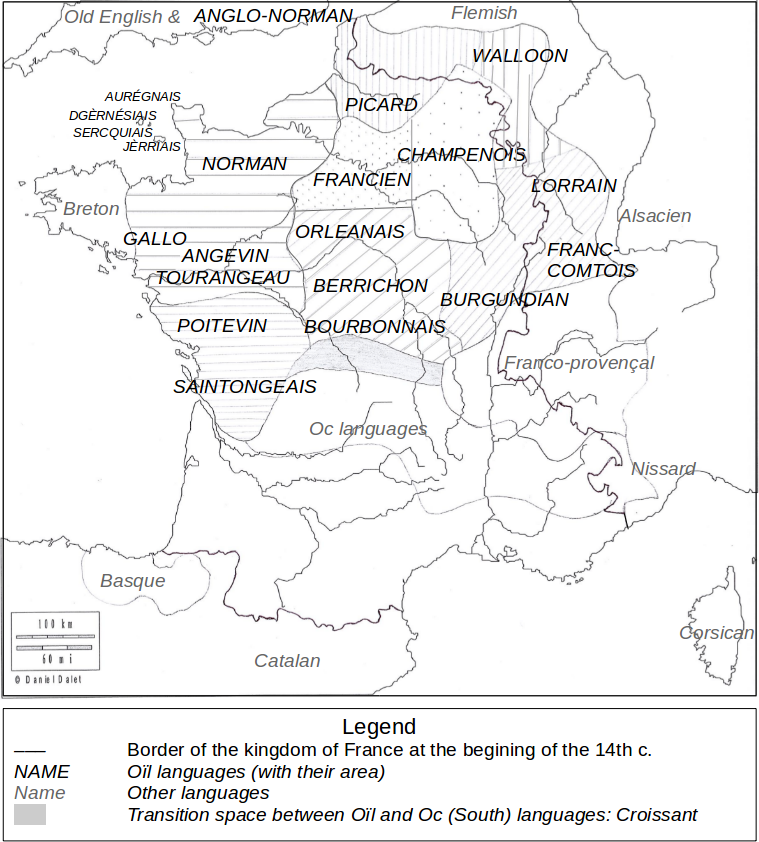
\includegraphics[scale=0.29]{static/media/mod_eval/bertrade/map-dialects2.png}
  \caption{Oïl languages}
  \label{fig:map-dialects}
\end{figure}

Medieval French covers both Old French (9th-13th c.) and Middle French (14th-15th c.). These stages are linguistically close and both precede the adoption of spelling norms. Middle French is more regular than Old French in some respects such as word order \citep{marchello-Nizia-etal-2020-grande} and less in others such as NP structure and pronouns system \citep{marchello-nizia-etal-1979-histoire}. Medieval French covers a set of \textit{Oïl} Romance languages spoken in the kingdom of France between the 9th and the 15th century (\cref{fig:map-dialects}).
There are around twenty such languages.

Older texts are close to Late Latin, and verse is prevalent until the end of the 13th century. Old French has a relatively free word order.
Until the mid-11th century, the prevalent order is \textit{Subject-Object-Verb} (SOV), which is then gradually supplanted by SVO, which is the default order in contemporary French. Unlike most languages with free word order, the functions of verbal arguments are not always given away by morphological clues, the already simplistic case system of Old French disappears progressively through the covered period.

There are also many cases of syntactic ambiguity. For example, in the following quote from \emph{Lancelot},\footnote{In the edition from Pierre Kunstmann, from the online \textit{Base de français médiéval}: \url{http://catalog.bfm-corpus.org/CharretteKu}.} (verse ~5436),
both \enquote{la dame} and \enquote{Lancelot} could be the subject or the object of \enquote{Vit} and only the context enables the reader to understand that \enquote{la dame} is the subject.

\digloss{Dolant et pansif Lancelot Vit la dame}
{Mournful and meditative Lancelot saw the lady}
{The lady saw that Lancelot was mournful and meditative.}

Word order is also relatively free within constituents. For example, a noun modifier can be on the left or on the right of its governor, and it is not necessarily preceded by a preposition. In contemporary French, it can only appear on the right, and it is found without a preposition only in some cases like named entities. Because of the general free word order and the absence of punctuation in our treebank, this adds up to the ambiguity of the analysis.

In each of the following examples from the SRCMF corpus, the noun following \emph{roi} (\enquote{king}) has a different analysis: head of \emph{roi}, modifier, argument of the same verb or a different one, with no explicit marking:

\begin{center}
    % beroul. modifieur à gauche.
    \begin{dependency}[theme=simple]
        \begin{deptext}[row 2/.style={font=\small}]
            \textit{Fus} \& \textit{tu} \& \textit{donc} \& \textit{pus} \& \textit{a} \& \textit{la} \& \textbf{\textit{roi}} \& \textit{cort} \\
            %VERB \& PRON \& ADV \& ADV \& ADP \& DET \& NOUN \& NOUN \\
            Were \& you \& then \& no more \& at \& the \& king \& court \\
        \end{deptext}
        \depedge{8}{7}{nmod}
        \depedge[edge start x offset=0.5em]{8}{6}{det}
        \depedge[edge start x offset=1em]{8}{5}{case}
    \end{dependency}

    \raggedright
    \enquote{Then were you not at the king's court anymore?} (\emph{Beroul Tristan})
\end{center}

\begin{center}
    % Graal. modifieur à droite.
    \begin{dependency}[theme=simple]
        \begin{deptext}[row 2/.style={font=\small}]
            \textit{la} \& \textit{fille} \& \textit{au} \& \textit{riche} \& \textbf{\textit{roi}} \& \textit{pescheor} \\
            the \& daughter \& of the \& rich \& king \& fisher \\
        \end{deptext}
        \depedge{5}{6}{flat}
    \end{dependency}

    \raggedright
    \enquote{the daughter of the rich Fisher King} (\emph{Queste del Saint Graal})
\end{center}

\begin{center}
    % Roland. arguments du même verbe.
    \begin{dependency}[theme=simple]
        \begin{deptext}[row 2/.style={font=\small}]
            \textit{De} \& \textit{Guenelun} \& \textit{atent} \& \textit{li} \& \textbf{\textit{reis}} \& \textit{nuveles} \\
            From \& Ganelon \& waits \& the \& king \& news \\
        \end{deptext}
        \depedge{3}{5}{nsubj}
        \depedge[edge start x offset=-0.5em]{3}{6}{obj}
    \end{dependency}

    \raggedright
    \enquote{The king waits for news from Ganelon.} (\emph{Chanson de Roland})
\end{center}

\begin{center}
    % Graal. arguments de verbes différents, et absence de ponctuation.
    \begin{dependency}[theme=simple]
        \begin{deptext}[row 2/.style={font=\small}]
            \textit{Biax} \& \textit{sire} \& \textit{fet} \& \textit{li} \& \textbf{\textit{rois}} \& \textit{escu} \& \textit{vos} \& \textit{envoiera} \& \textit{Diex} \\
            Dear \& Sir \& says \& the \& king \& shield \& you \& send-FUT \& God \\
        \end{deptext}
        \depedge{3}{5}{nsubj}
        \depedge{8}{6}{obj}
    \end{dependency}

    \raggedright
    \enquote{Dear Sir, says the king, God will send you a shield.} (\emph{Queste del Saint Graal})
\end{center}

Furthermore, overt subjects are not mandatory, and are often dropped in texts written in verse until the 12th century, after which the presence of subjects increases through time.
These phenomena are particularly prevalent in verse, where metric and rhyming constraints often lead to more contrived syntactic forms than in prose.

Another source of ambiguity is the variety of spellings, due to the lack of spelling standard. For example, the word \textit{moult} (transl. \textit{a lot (of), very}), emblematic of this period, is initially an adjective, and it is progressively grammaticalized, becoming an adverb. Several forms appear at the same time, some with a declension, some without, and the radical does not have a fixed spelling: \textit{molt(e)(s), molz, mult(e)(s), mul(t)z, mou(l)t}…

\subsection{Early Modern French}\label{def:early}

\begin{table*}[!htp]
    \centering\small
    \begin{tabular}{@{}p{0.3\linewidth}p{0.3\linewidth}p{0.3\linewidth}@{}}
        \toprule
        Source                                                                                                                                                                                                                                                                                               & Normalised & Translation \\
        \midrule
        Surquoy, SIRE, s’il plaiſt à voſtre Maieſté de ſe ſouuenir des miſeres de ſon Eſtat, dõt au moins ell’a tiré cét aduantage, qu’en vne grande ieuneſse ell’a acquis vne grande experi\~ece, elle verra que tous les mal-heurs de sõ bas âge ont pris leur commencement en ſemblables occaſions;       &
        \emph{Sur quoi, SIRE, s’il plaît à votre Majesté de se souvenir des misères de son état dont au moins elle a tiré cet avantage, qu’en une grande jeunesse elle a acquis une grande expérience, elle verra que tous les malheurs de son bas âge ont pris leur commencement en semblables occasions~;} &
        \textcolor{gray}{``Whereupon, SIR, if it pleases your Majesty to remember the miseries of her state, from which at least she has derived this advantage, that in great youth she has acquired great experience, she will see that all the misfortunes of her early life took their beginning on similar occasions;''}           \\
        \bottomrule
    \end{tabular}
    \caption{\label{tab:norm_examples}Example of normalisation taken from the \emph{Lettres} of \protect\newcite{balzac-1624-lettres}.}
\end{table*}

We loosely define Early Modern French as a state of language following Middle French in 1500---following here the \emph{terminus ad quem} used by the \emph{Dictionnaire de Moyen Français} \cite{martin-2020-dictionnaire}---and ending with the French Revolution in 1789. It therefore encompasses three centuries (16\textsuperscript{th}, 17\textsuperscript{th} and 18\textsuperscript{th}\,c.), or two linguistic periods: the \emph{français préclassique} or ``preclassical French'', 1500--1630 and the \emph{français classique} or ``classical French'', 1630--1689; both periodisations are currently used in French linguistics (\emph{e.g.}~by \newcite{vachon-2010-changement} and \newcite{amatuzzi-etal-2019-ameliorer}).

A typical example of Early Modern French, taken from ~\newcite{balzac-1624-lettres}, is given in Table~\ref{tab:norm_examples}. We note here the presence of several phenomena that have now disappeared in contemporary French, such as the presence of abbreviations (\emph{dõt}$\to$\emph{dont}), the long \emph{s} (\emph{ſ}, see\,\emph{miſeres}), the use of \emph{v} instead of \emph{u} (\emph{vne} for \emph{une}), the conservation of etymological letters (\emph{voſtre}$<$Latin~\emph{vŏster} rather than \emph{votre}) and calligraphic letters (\emph{-y} in \emph{Surquoy}), the absence of welding  (\emph{\mbox{mal-heurs}} and not \emph{malheurs}) and the opposite (\emph{Surquoy} and not \emph{Sur quoi}).

For NLP tasks, which process raw sequences, such differences with respect to contemporary French are not trivial, and they prevent the processing of historical texts with tools trained on recent sources.

\section{Outline}

